

\chapter{LSD SLAM}
\section{程序流程}

整个程序大致有4个线程(一些能够并行的任务也用来了线程池来计算):

分别是主线程用来追踪每一帧的位姿,并决定是否创建关键帧,流程如图\ref{fig:tracking}所示;

mappingThreadLoop线程,用来构建新的深度图或者是更新当前关键帧的深度图,流程如图\ref{fig:mapping_thread}所示;

constraintSearchThreadLoop线程,用来除当前关键帧之外的那些关键帧是否存在闭环,如果存在闭环,则生成pose graph的约束关系,并插入到pose graph中,流程如图\ref{fig:constraint_search_thread}所示;

optimizationThreadLoop线程,用来对已经构建的位姿图进行优化,流程如图\ref{fig:mapping_thread}所示。


\begin{figure}[h]%%图
	\centering  %插入的图片居中表示
	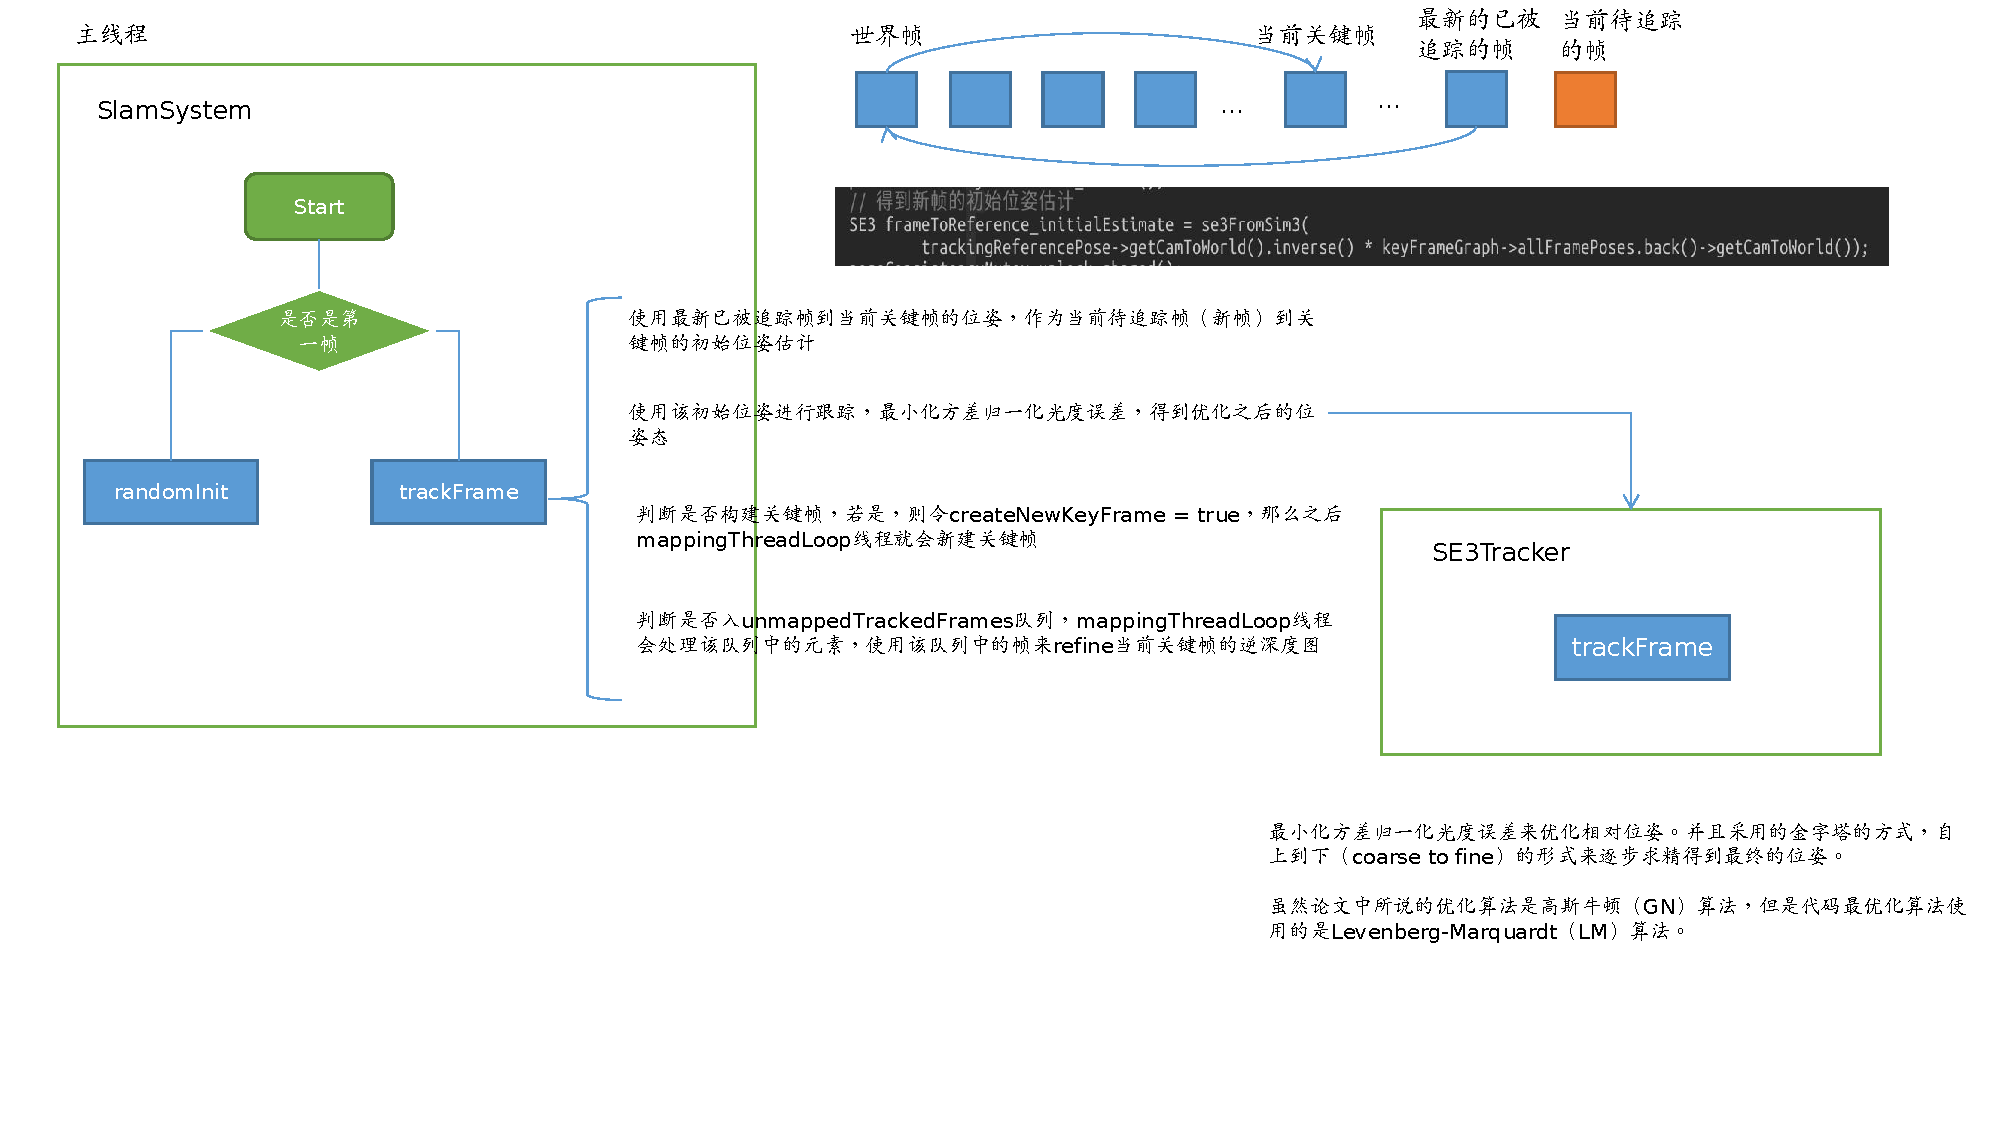
\includegraphics[width=1.0\linewidth]{image/LSD-SLAM/LSD-SLAM-tracking.pdf}  %插入的图,包括JPG,PNG,PDF,EPS等,放在源文件目录下
	\caption{跟踪流程图.}  %图片的名称
	\label{fig:tracking}   %标签,用作引用
\end{figure}





\begin{figure}[h]%%图
	\centering  %插入的图片居中表示
	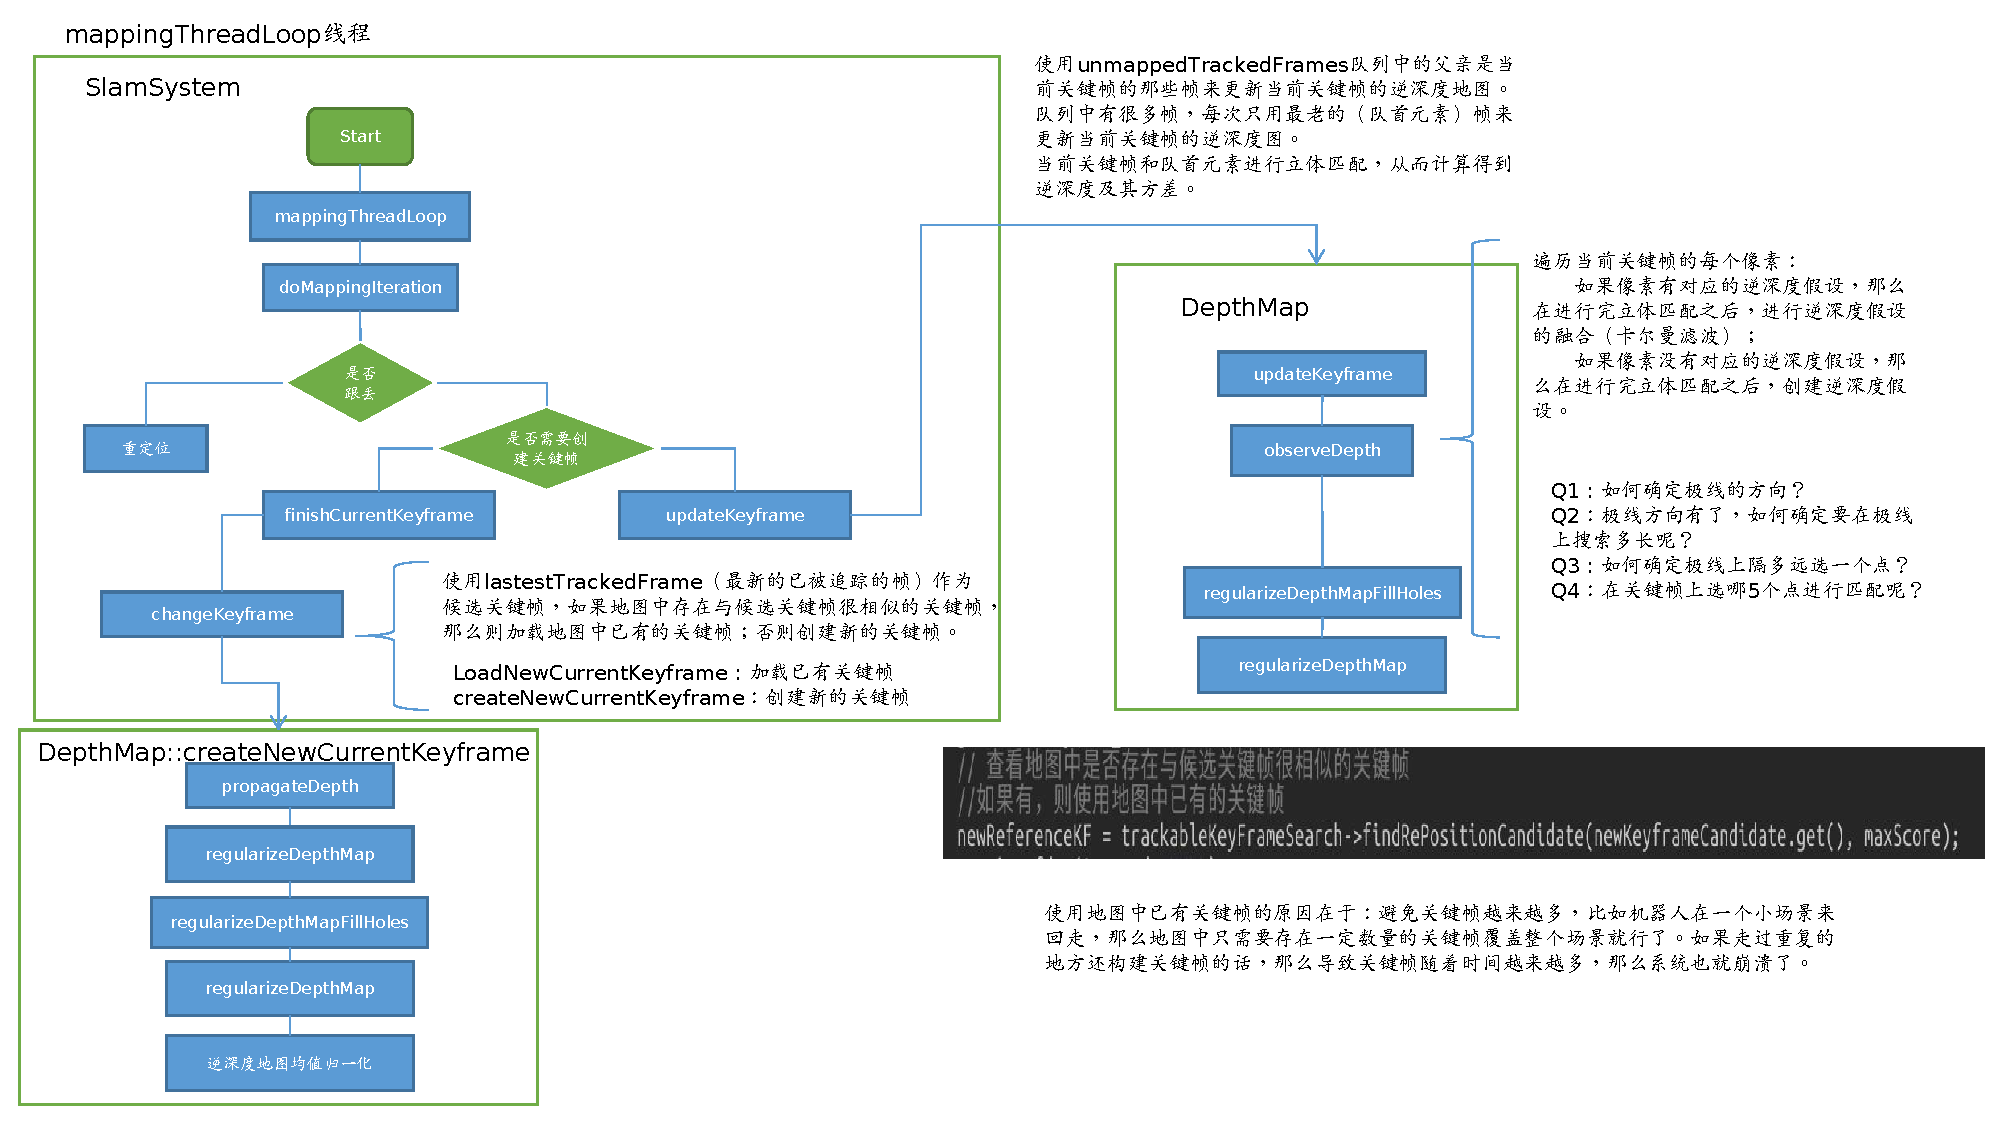
\includegraphics[width=1.0\linewidth]{image/LSD-SLAM/LSD-SLAM-mapping}  %插入的图,包括JPG,PNG,PDF,EPS等,放在源文件目录下
	\caption{mappingThreadLoop流程图.}  %图片的名称
	\label{fig:mapping_thread}   %标签,用作引用
\end{figure}



\section{Tracking}
\subsection{公式推导}
\subsubsection{归一化光度误差}
	LSD SLAM的帧间追踪,也是基于直接法的一般套路,使用前一帧到参考帧的相对位姿作为参考帧到当前帧相对位姿的初始估计(基于小运动假设),然后通过最小化光度误差(photometric error)来得到优化过后的位姿态。
	
	不过,LSD SLAM在一般光度误差的基于上进行了改善,使用的是方差归一化光度误差(variance-normalized photometric error)
\begin{equation}
E_p(\bm{\xi}_{ji}) = \sum_{p \in \Omega_{D_i}}\| \frac{r_p^2(\bm{p}, \bm{\xi}_{ji})}{\sigma_{r_p}^{2}(\bm{p}, \bm{\xi}_{ji})} \|_\delta
\end{equation}

其中
\begin{equation}
	r_p(\bm{p},\bm{\xi}_{ji}) := I_i(\bm{p}) - I_j(\omega(\bm{p}, D_i(\bm{p}), \bm{\xi}_{ji}))
\end{equation}

\begin{equation}
	\sigma_{r_p}^{2}(\bm{p}, \bm{\xi}_{ji}) := 2\sigma_I^2 + (\frac{\partial r_p(\bm{p}, \bm{\xi}_{ji})}{\partial D_i(\bm{p})})^2V_i(\bm{p})
\end{equation}

这里的$||*||_\delta$为Huber-norm,表示为:
\begin{equation}
	||r^2||_\delta := 
		\begin{cases}
			\frac{r^2}{2\delta} &  if \ \ |r| \le \delta \\
			|r| - \frac{\delta}{2} & otherwise\\
		\end{cases}
\end{equation}

式子中的$\bm{\xi}_{ji}$就是要求得两帧之间的SE3变换(从$i \rightarrow j$,也就是参考帧到当前帧的变换),这里使用李代数的形式表示;这里的$\bm{p}$是在参考帧$I_i$下观测到的有深度信息($\bm{p} \in \Omega_{D_i}$)的\textbf{归一化相机平面上的点};函数$D_i(\bm{p})$是点$p$在参考帧下的\textbf{逆深度},$V_i(\bm{p})$是对应的逆深度的方差;函数$\omega(\bm{p}, D_i(\bm{p}), \bm{\xi}_{ji})$则是将参考帧下的图像像素坐标根据逆深度反向投影得到3D点,然后将3D点投影到当前帧的图像平面;这里的$\sigma_I^2$是图像的高斯噪声。

\begin{note}
	以上公式都省略了相机内参,也即省略了归一化相机平面坐标到图像像素平面坐标的转换($ \bm{u} = \bm{K}\bm{p}$),但是在LSD SLAM的代码中是不会省略的。
\end{note}


论文在计算两帧之间位姿变换时,将所有有逆深度假设的像素都用上了。但是每个逆深度的确定性不同,也就是有些逆深度比较准确(方差$V_i(\bm{p})$小),有些不准确(方差$V_i(\bm{p})$大)。因此在公式(1.1)中在残差上除以方差做了归一化。方差的第一项是两个图像的高斯噪声,第二项则是使用了方差传播公式计算得到的,即由于误差是使用\textbf{逆深度}计算得到的,那么逆深度的方差就会传播到误差的方差。所以将光度误差除以其方差,就得到了方差归一化的光度误差,这里应该是利用了马氏距离的思想。


公式(1.1)、(1.2)、(1.3)、(1.4)就是LSD计算位姿时,所使用的误差函数,公式中的大部分都比较简单,且在其它SLAM都有的东西,主要是公式(1.3)中误差中\textbf{逆深度}的求导是比较新的东西,下面对其导数进行推导:


%\begin{align*}
%	&\frac{\partial [I_i(\bm{p}) - I_j(\omega(\bm{p}, D_i(\bm{p}), \bm{\xi}_{ji}))]}{\partial D_i(\bm{p})} \\
%	&= - \frac{\partial I_j(\omega(\bm{p}, D_i(\bm{p}), \bm{\xi}_{ji}))}{\partial D_i(\bm{p})} \\
%	&= -\frac{\partial I_j(\bm{u}')}{\partial \bm{u}'} \frac{\partial \bm{u}'}{\partial \bm{p}'} \frac{\partial \bm{p}'}{\partial \bm{X}'} \frac{\partial \bm{X}'}{\partial D_i(\bm{p})}
%\end{align*}


首先,列出一些必要的公式
\begin{equation}
\bm{u} = \bm{K} \bm{p}
\end{equation}

\begin{equation}
\bm{u}' = \bm{K} \bm{p}'
\end{equation}

\begin{equation}
\bm{X} = \frac{1}{D_i(\bm{p})} \bm{p} =  \frac{1}{D_i(\bm{p})} \bm{K}^{-1} \bm{u}
\end{equation}

\begin{equation}
\bm{X}' = R \frac{1}{D_i(\bm{p})} \bm{K}^{-1} \bm{u} + t
\end{equation}


其中$\bm{u}'$是参考帧图像$I_i$的像素平面坐标点$\bm{u}$在当前帧图像$I_j$下的对应点;$\bm{X}'$则是点$\bm{u}'$在当前帧相机坐标系下所对应的3D点,该3D点是参考帧图像$I_i$的归一化平面点$\bm{p}$根据逆深度$D_i(\bm{p})$反向投影,然后根据位姿$\bm{\xi}_{ji}$旋转平移得到的.


那么根据链式法则,能够得到下面的导数:


\begin{equation}
	\begin{split}
		&\frac{\partial [I_i(\bm{p}) - I_j(\omega(\bm{p}, D_i(\bm{p}), \bm{\xi}_{ji}))]}{\partial D_i(\bm{p})} \\
		&= - \frac{\partial I_j(\omega(\bm{p}, D_i(\bm{p}), \bm{\xi}_{ji}))}{\partial D_i(\bm{p})} \\
		&= -\frac{\partial I_j(\bm{u}')}{\partial \bm{u}'} \frac{\partial \bm{u}'}{\partial \bm{X}'}  \frac{\partial \bm{X}'}{\partial D_i(\bm{p})}
	\end{split}
\end{equation}







导数的第一项是图像梯度:
\begin{equation}
\frac{\partial I_j(\bm{u}')}{\partial \bm{u}'} = 
	\left[
	\begin{array}{cc}
		gx & gy
	\end{array}
	\right]
\end{equation}

根据公式(1.7)知道$\bm{X}'$是如何计算得到$\bm{u}'$的,从而得到导数的第二项如公式(1.8)所示:

\begin{equation}
	\bm{u}' = \left[ \begin{array}{c}
		u' \\
		v'
	\end{array}\right] 
	= \frac{1}{Z'}  
		\left[ \begin{array}{ccc}
			fx & 0 & cx \\
			 0 & fy& cy \\
			 0 & 0 & 1 
		\end{array}\right]
		\left[ \begin{array}{c}
			X' \\
			Y' \\
			Z' 
		\end{array}
		\right]
	= \left[ \begin{array}{c}
		(fx X' + cx) / Z' \\
		(fy Y' + cy) / Z' \\
	\end{array}\right]
\end{equation}


\begin{equation}
	\frac{\partial \bm{u}'}{\partial \bm{X}'}
	=
	\left[ 
		\begin{array}{ccc}
			\frac{fx}{Z'} & 0 & -\frac{fxX'}{Z'^2} \\
			0 & \frac{fy}{Z'} & -\frac{fyY'}{Z'^2} 
		\end{array}
	\right]
\end{equation}


根据公式(1.9)知道$\bm{X}'$是如何根据$\bm{p}$、逆深度$D_i(\bm{p})$以及位姿$\bm{\xi}_{ji}$计算得到的,所以导数的第三项如公式(1.10)所示:


\begin{equation}
	\frac{\partial \bm{X}'}{\partial D_i(\bm{p})}
	=
	-\frac{1}{D_i(\bm{p})^2}\bm{R}\bm{K}^{-1} \bm{u}
\end{equation}

进行进一步推导,能够得到:

\begin{equation}
	\bm{X}' = \frac{1}{D_i(\bm{p})} \bm{R} \bm{K}^{-1}\bm{u} + \bm{t}
\end{equation}
\begin{equation}
	-\bm{X}' = -\frac{1}{D_i(\bm{p})} \bm{R} \bm{K}^{-1}\bm{u} - \bm{t}
\end{equation}
\begin{equation}
	\bm{t} -\bm{X}' = -\frac{1}{D_i(\bm{p})} \bm{R} \bm{K}^{-1}\bm{u}
\end{equation}

\begin{equation}
\frac{\bm{t} -\bm{X}'}{D_i(\bm{p})} = -\frac{1}{D_i(\bm{p})^2} \bm{R} \bm{K}^{-1}\bm{u}
\end{equation}
\begin{equation}
		\frac{\partial \bm{X}'}{\partial D_i(\bm{p})} = \frac{\bm{t} -\bm{X}'}{D_i(\bm{p})}
		= 
		\frac{1}{D_i(\bm{p})}
		\left[
			\begin{array}{c}
				t_x - X' \\
				t_y - Y' \\
				t_z - Z'
			\end{array}
		\right]
\end{equation}



综上所述,得到最终的导数是:
\begin{equation}
\begin{split}
	&-\left[
		\begin{array}{cc}
			gx & gy
		\end{array}
	\right]
	\left[ 
		\begin{array}{ccc}
			\frac{fx}{Z'} & 0 & -\frac{fxX'}{Z'^2} \\
			0 & \frac{fy}{Z'} & -\frac{fyY'}{Z'^2} 
		\end{array}
	\right]		
	\frac{1}{D_i(\bm{p})}
	\left[
		\begin{array}{c}
			t_x - X' \\
			t_y - Y' \\
			t_z - Z'
		\end{array}
	\right] \\
	&=
	-\left[
		\begin{array}{cc}
			gx fx &	gy fy
		\end{array} 
	\right]
	\left[ 
		\begin{array}{c}
			\frac{t_x - X'}{Z'D_i(\bm{p})^2}- \frac{(t_z - Z')X'}{Z'^2 D_i(\bm{p})}\\
			\frac{t_y - Y'}{Z'D_i(\bm{p})^2}- \frac{(t_z - Z')Y'}{Z'^2 D_i(\bm{p})}\\
		\end{array}
	\right]
\end{split}
\end{equation}


通分,整理合并之后,得到LSD SLAM代码中误差光度误差关于逆深度$D_i(\bm{p})$的导数为:

\begin{equation}
\begin{split}
&\frac{\partial [I_i(\bm{p}) - I_j(\omega(\bm{p}, D_i(\bm{p}), \bm{\xi}_{ji}))]}{\partial D_i(\bm{p})} \\
&=
-\left[
\begin{array}{cc}
gx fx & gy fy
\end{array} 
\right]
\left[ 
\begin{array}{c}
\frac{txZ' - tzX'}{Z'^2D_i(\bm{p})}\\
\frac{tyZ' - tzY'}{Z'^2D_i(\bm{p})}\\
\end{array} 
\right]
\end{split}
\end{equation}




参考 : \href{https://zhuanlan.zhihu.com/p/54129298}{LSD-SLAM权重更新公式推导}




\subsubsection{加权最小二乘法}


\begin{equation}
E_p(\bm{\xi}_{ji}) = \sum_{p \in \Omega_{D_i}}\| I_i(\bm{p}) - I_j(\omega(\bm{p}, D_i(\bm{p}), \bm{\xi}_{ji}))  \|^2
\end{equation}

\begin{equation}
	\min_{\bm{\xi}_{ji}} E_p(\bm{\xi}_{ji})
\end{equation}
普通最小二乘法就是直接最小化该误差,从而得到优化过有的位姿。由附录\ref{appendix:non-linear-least-square}可得该非线性最小二乘的解如下:
\begin{equation}
	\delta \bm{\xi}_{ji}^{(n)} = -(J^TJ)^{-1} J^Tr(\bm{\xi}_{ji}^{(n)})
\end{equation}

位姿的更新公式为:
\begin{equation}
	\bm{\xi}_{ji}^{(n+1)} = \delta \bm{\xi}_{ji}^{(n)} \circ \bm{\xi}_{ji}^{(n)}
\end{equation}




为了减少外点的影响,例如由于遮挡(occlusions)和镜面反射(reflections)所导致的错误的点对应,作者使用了加权最小二乘,在每次迭代时,计算权重$\bm{W}=\bm{W}(\bm{\xi}_{ji}^{(n)})$。
所以误差函数变为:
\begin{equation}
	E_p(\bm{\xi}_{ji}) = \sum_{p \in \Omega_{D_i}} w_p(\bm{\xi}_{ji}) \| I_i(\bm{p}) - I_j(\omega(\bm{p}, D_i(\bm{p}), \bm{\xi}_{ji}))  \|^2
\end{equation}
从而最小二乘的解变为:
\begin{equation}
		\delta \bm{\xi}_{ji}^{(n)} = -(J^TWJ)^{-1} J^TWr(\bm{\xi}_{ji}^{(n)})
\end{equation}

该权重就是误差的方差的倒数,并经过Huber-norm进行加权,也即公式(1.3)与公式(1.4)。
需要注意的是,在代码的实现中误差并没有经过Huber-norm进行加权。这与公式(1.1)不符。

\subsection{代码解析}




LSD SLAM通过最小化方差归一化光度误差来求解两帧图像之间的位姿变化,并且采用了LM算法迭代求解。LSD SLAM求解两帧图像的SE3变换的函数主要在\textbf{SE3Tracker}中实现中。该类中有四个函数比较重要,分别为

\begin{itemize}
	\item \href{https://github.com/tum-vision/lsd_slam/blob/catkin/lsd_slam_core/src/Tracking/SE3Tracker.cpp#L280}{SE3Tracker::trackFrame}
	\item \href{https://github.com/tum-vision/lsd_slam/blob/catkin/lsd_slam_core/src/Tracking/SE3Tracker.cpp#L885}{SE3Tracker::calcResidualAndBuffer}
	\item \href{https://github.com/tum-vision/lsd_slam/blob/catkin/lsd_slam_core/src/Tracking/SE3Tracker.cpp#L749}{SE3Tracker::calcWeightsAndResidual}
	\item \href{https://github.com/tum-vision/lsd_slam/blob/catkin/lsd_slam_core/src/Tracking/SE3Tracker.cpp#L1277}{SE3Tracker::calculateWarpUpdate}
\end{itemize}


\begin{lstlisting}[language = C++]
SE3 SE3Tracker::trackFrame(
	TrackingReference* reference,
	Frame* frame,
	const SE3& frameToReference_initialEstimate);
\end{lstlisting}

函数\textbf{SE3Tracker::trackFrame}需要传入三个形参,从参考帧到当前帧,首先是两帧图像帧的实例,另外就是给定的两帧之间的\textbf{初始相对位姿},对于\textbf{初始相对位姿},LSD SLAM使用了上一帧到参考帧的位姿作为当前位姿估计的初始值。

\textbf{SE3Tracker::trackFrame}函数的主体是一个for循环,从金字塔的高层开始遍历知道底层。在循环内使用加权高斯牛顿法算法(Weighted Gauss-Newton Optimization)来对位姿进行优化,并使用金字塔上一层优化过后的位姿作为下一层的初始位姿。该函数的代码结构可以归纳如下:


\begin{lstlisting}
从上到下遍历金字塔的每一层
step1 : 对参考帧当前层构造点云(reference->makePointCloud)
step2 : 使用也有的位姿估计计算残差以及一些所需要的数据,并存放到buffer中(calcResidualAndBuffers)
step3 : 计算残差的权重,也即残差的方差的倒数(calcWeightAndResidual)
step4 : 计算每个残差的雅克比向量,并更新A和b(calculateWarpUpdate)
step5 : 计算得到增量inc = A.ldlt().solve(b)

\end{lstlisting}



在GN优化时,在每次迭代之后都要重新计算雅克比矩阵、残差以及权重矩阵。雅克比矩阵和残差在函数\textbf{SE3Tracker::calcResidualAndBuffers}中计算,而权重矩阵(实际上是权重系数)在\textbf{SE3Tracker::calcWeightAndResidual}中计算。接着在函数\textbf{SE3Tracker::calculateWarpUpdate}中构造方重组,最后求解方程组。


作者论文中说的是GN优化算法,但是代码中实际使用的是LM算法优化,LM算法的区别于GN算法的地方在于求解最小二乘$Ax=b$的时候,增加了一个系数$\lambda$,也就是$(A+\lambda I)x=b$。$\lambda$越大,越接近梯度下降法。 在代码中,如果此次迭代收敛(此次误差相对于前一次的误差减少了),那么减少$\lambda$的权重,如果此次迭代不收敛(此次误差相对于前一次的误差增大了),那么增大$\lambda$的权重。


更加详细的源码阅读,可以看这篇笔记:\href{https://www.zybuluo.com/kokerf/note/855220}{LSD-SLAM笔记之SE3Tracking};或者是这篇笔记:\href{https://www.baidu.com/link?url=gFb5QHUu2_4TmXHqie8m0oBYpXRHrJXFhlNW8pf9i-HOnoGS7nJXVs7YlJ88vmNC&wd=&eqid=f3e75ce0000ca6a5000000035c76477c}{LSD-SLAM解读——帧间追踪(详细推导)}


\section{DepthMap}
	
LSD SLAM构建的地图是半稠密逆深度地图(semi-dense inverse depth map),只对有明显梯度的像素位置进行深度估计,用逆深度表示,并且假设逆深度的噪声服从高斯分布。


\subsection{极线搜索的尺度问题}
LSD SLAM在当前关键帧上取5点,然后在参考帧上沿着极线移动,也取5点进行匹配。那么存在如下几个问题是需要想明白的:

\begin{enumerate}
	\item Q1 : 在关键帧上取哪5个点呢?
	\item Q2 : 在参考帧上,沿着极线取间隔多大的5个点呢?
	\item Q3 : 
\end{enumerate}



首先,我们分析一下二视图立体几何是如何计算视差图的。例如:对于左图中y = 5这行上的每个点x,只需要在右图中y = 5这行上进行极线搜索就行了。进一步进行分析,左图中y = 5这行上的每个点x,其在右图中的极线都是相同的,也即都是右图中y = 5这条直线;同理,右图中y = 5这行上的每个点x,其在左图中的极线也都是相同的,也即都是左图中y = 5这条直线。
\begin{note}
	这里应该有一张二视图视差搜索图。
\end{note}

将上面的结论推广到未进行极线矫正的两张图像上,左图中一条极线上的点,在右图中的极线都是相同的;同理,右图中一条极线上的点,在左图中的极线也是相同的。也就是说左图极线上的某些点,与右图极线上的某些点是匹配点。

所以,LSD SLAM对于在当前关键帧上的每个点$u$在参考帧上进行极线搜索时,是这么做的:

\begin{enumerate}
	\item 计算当前关键帧上的点$u$在参考帧上所对应的极线;
	\item 计算参考帧上的极线在当前关键帧上所对应的极线,由于过两点确定一条直线,在当前关键帧上对应的极线过点$u$和极点$e$
	\item 在当前关键帧上,在点$u$的附近按照极线方向,按照一定的距离,取5个点;
	\item  在参考帧上,沿着极线方向进行搜索,每次取间隔为单位长度1的5个点进行匹配。
	\item cost最小的点,就是匹配点。
\end{enumerate}


可能会有一个疑问就是,能够保证左图中过点$u$的极线只有一条吗。如果过点$u$的极线有多条,那么上面的方法算出来的极线可能不是我们想要的。这个担忧是没有必要的,\textbf{极线相交于极点,所以,对于非极点的像素点,其只会位于一条极线上,因为两条直线不可能相交于两点}。

\begin{note}
	如果点$u$和极点$e$非常接近,那么过点$u$的极线可能就不止一条了。这是因为所有的极线都过极点$e$,又因为$u$和极点$e$非常接近,所以导致过点$u$的极线可能不止一条了。所以说,如果点$u$和极点$e$非常接近时,根据上面的方法计算得到的极线方向可能是不稳定的,所以不能要。所以,LSD SLAM的代码中,也有对得到的极线长度的平方进行判断,如果太短了,小于1,那么就认为不稳定。
\end{note}



已知参考帧到当前关键帧的相对旋转和平移为$R$和$t$,也即默认参考帧为世界坐标系的情况下,参考帧的光心在当前关键帧下的坐标为:
\begin{equation}
	O = R \left[\begin{array}{c}
		0 \\
		0 \\
		0
	\end{array}\right] + t = t
\end{equation}

参考帧的光心在当前关键帧上的投影为
\begin{equation}
	e = KO = 
		\frac{1}{o_z}\left[ 
			\begin{array}{ccc}
			f_x & 0 & c_x \\
			0 & f_y & c_y \\
			0 & 0 & 1
			\end{array}
		\right] 
		\left[ 
			\begin{array}{c}
				o_x \\
				o_y \\
				o_z 
			\end{array}
		\right]
		=
		\frac{1}{o_z} 
		\left[
			\begin{array}{c}
				f_x o_x + c_x o_z \\
				f_y o_y + c_y o_z \\
				o_z
			\end{array}
		\right]
		=
		\left[
			\begin{array}{c}
				\frac{1}{o_z}(f_x o_x + c_x o_z) \\
				\frac{1}{o_z}(f_y o_y + c_y o_z) \\
				1
			\end{array}
		\right]		
\end{equation}

两点确定一条直线,从而点$u$在\textbf{当前关键帧}上的极线为
\begin{equation}
	l = u - e = 
	\left[
		\begin{array}{c}
			x \\
			y
		\end{array}
	\right]
	- 
	\frac{1}{o_z}
	\left[
		\begin{array}{c}
			f_x o_x + c_x o_z  \\
			f_y o_y + c_y o_z
		\end{array}
	\right]
	= 
	\frac{1}{o_z}
	\left[
		\begin{array}{c}
			-f_x o_x + o_z (x - c_x) \\
			-f_y o_y + o_z (y - c_y)
		\end{array}
	\right]
\end{equation}




下面解决,两条极线之间的尺度问题,也就是图像的“畸变”。比如,左图离场景1m,而右图距离场景2m,那么左图极线上的2个像素就对应于右图极线上的1个像素。所以在左极线上搜索时,可能每次要跨越2个像素。当然了,这是在没有考虑旋转,只有平移的情况下的推导。


首先,规定在参考帧上沿着极线搜索的距离为单位距离$incx^2 + incy^2 = 1$,那么要做的就是确定右图中沿着极线跨越了一个单位距离,在左图中跨越的距离。设在参考帧上跨越单位距离的两个点为$p_1$和$p_2$,这两个点在当前关键帧上的匹配点为$p_1'$和$p_2'$,那么要做的就是计算得到$p_1'$和$p_2'$的距离。

\begin{equation}
	P_1 = \frac{1}{d_r} K^{-1}  
	\left[ 
	\begin{array}{c}
		p_1 \\
		1
	\end{array}
	\right]
\end{equation}
\begin{equation}
	P_2 
	= 
	\frac{1}{d_r} K^{-1}  
	\left[
	\begin{array}{c}
	p_2\\
	1
	\end{array}
	\right]
	= \frac{1}{d_r} K^{-1}  
	\left[
	\begin{array}{c}
	p_1 + l_r\\
	1
	\end{array}
	\right]
\end{equation}

将参考帧中相距单位距离的两个点分别变换到当前关键帧的坐标系下:
\begin{equation}
	\frac{1}{d_k}K^{-1} 
	\left[
		\begin{array}{c}
			p_1' \\
			1
		\end{array}
	\right] 
	= R \frac{1}{d_r} K^{-1} 
	\left[
		\begin{array}{c}
			p_1 \\
			1
		\end{array}
	\right]
	+ t
\end{equation}

\begin{equation}
\frac{1}{d_k}K^{-1} 
\left[
\begin{array}{c}
p_2' \\
1
\end{array}
\right] 
= R \frac{1}{d_r} K^{-1} 
\left[
\begin{array}{c}
p_1  + l_r\\
1
\end{array}
\right]
+ t
\end{equation}

两式相减,并整理,得到:
\begin{equation}
	\left[
		\begin{array}{c}
			p_2' - p_1'\\
			0
		\end{array}
	\right]
	=
	\frac{d_k}{d_r}KRK^{-1}	
	\left[
		\begin{array}{c}
			l_r \\
			0
		\end{array}
	\right]
\end{equation}
从而得到$p_1'$和$p_2'$的距离为:

\begin{equation}
	\|p_2' - p_1' \| = \| \frac{d_k}{d_r} \| \| K R K^{-1}\| \| l_r \| \approx \frac{d_k}{d_r}
\end{equation}
也就是说当旋转比较小(接近单位矩阵)时,$p_1'$和$p_2'$的距离为$\frac{d_k}{d_r}$。从而知道当前关键帧上的点$u$沿着极线,隔多远的距离进行取点。



\begin{note}
	注意这里的$d_k$和$d_r$是逆深度,将逆深度换成深度就更好理解了,也更加直观。
\end{note}








\section{Constraint Search}

Tracking线程负责追踪下一帧图像的位姿,并且负责判断是否需要创建关键帧,如果需要,那么令$createNewKeyFrame = true$。Mapping线程会根据该变量来决定是否创建关键帧,如果创建关键帧,那么就会利用当前关键帧所追踪到的那些帧来更新当前关键帧的地图;如果要创建关键帧,那么将当前关键帧插入到Constratint Search线程的newKeyFrames队列中,然后创建新的关键帧。

也就是说newKeyFrame队列中都是以往的关键帧,如果newKeyFrame队列不为空,那么就会取队列的第一帧进行Constraint Search;如果newKeyFrame队列为空,那么就会随机挑选关键帧进行Constraint Search。


Constraint Search就是对关键帧找到其\textbf{相似}的关键帧,然后在这些相似的关键帧中挑选中通过双向\textbf{SE3}和\textbf{Sim3}测试的帧,然后生成两帧之间的约束关系,然后插入到pose graph中。


\begin{figure}[h]%%图
	\centering  %插入的图片居中表示
	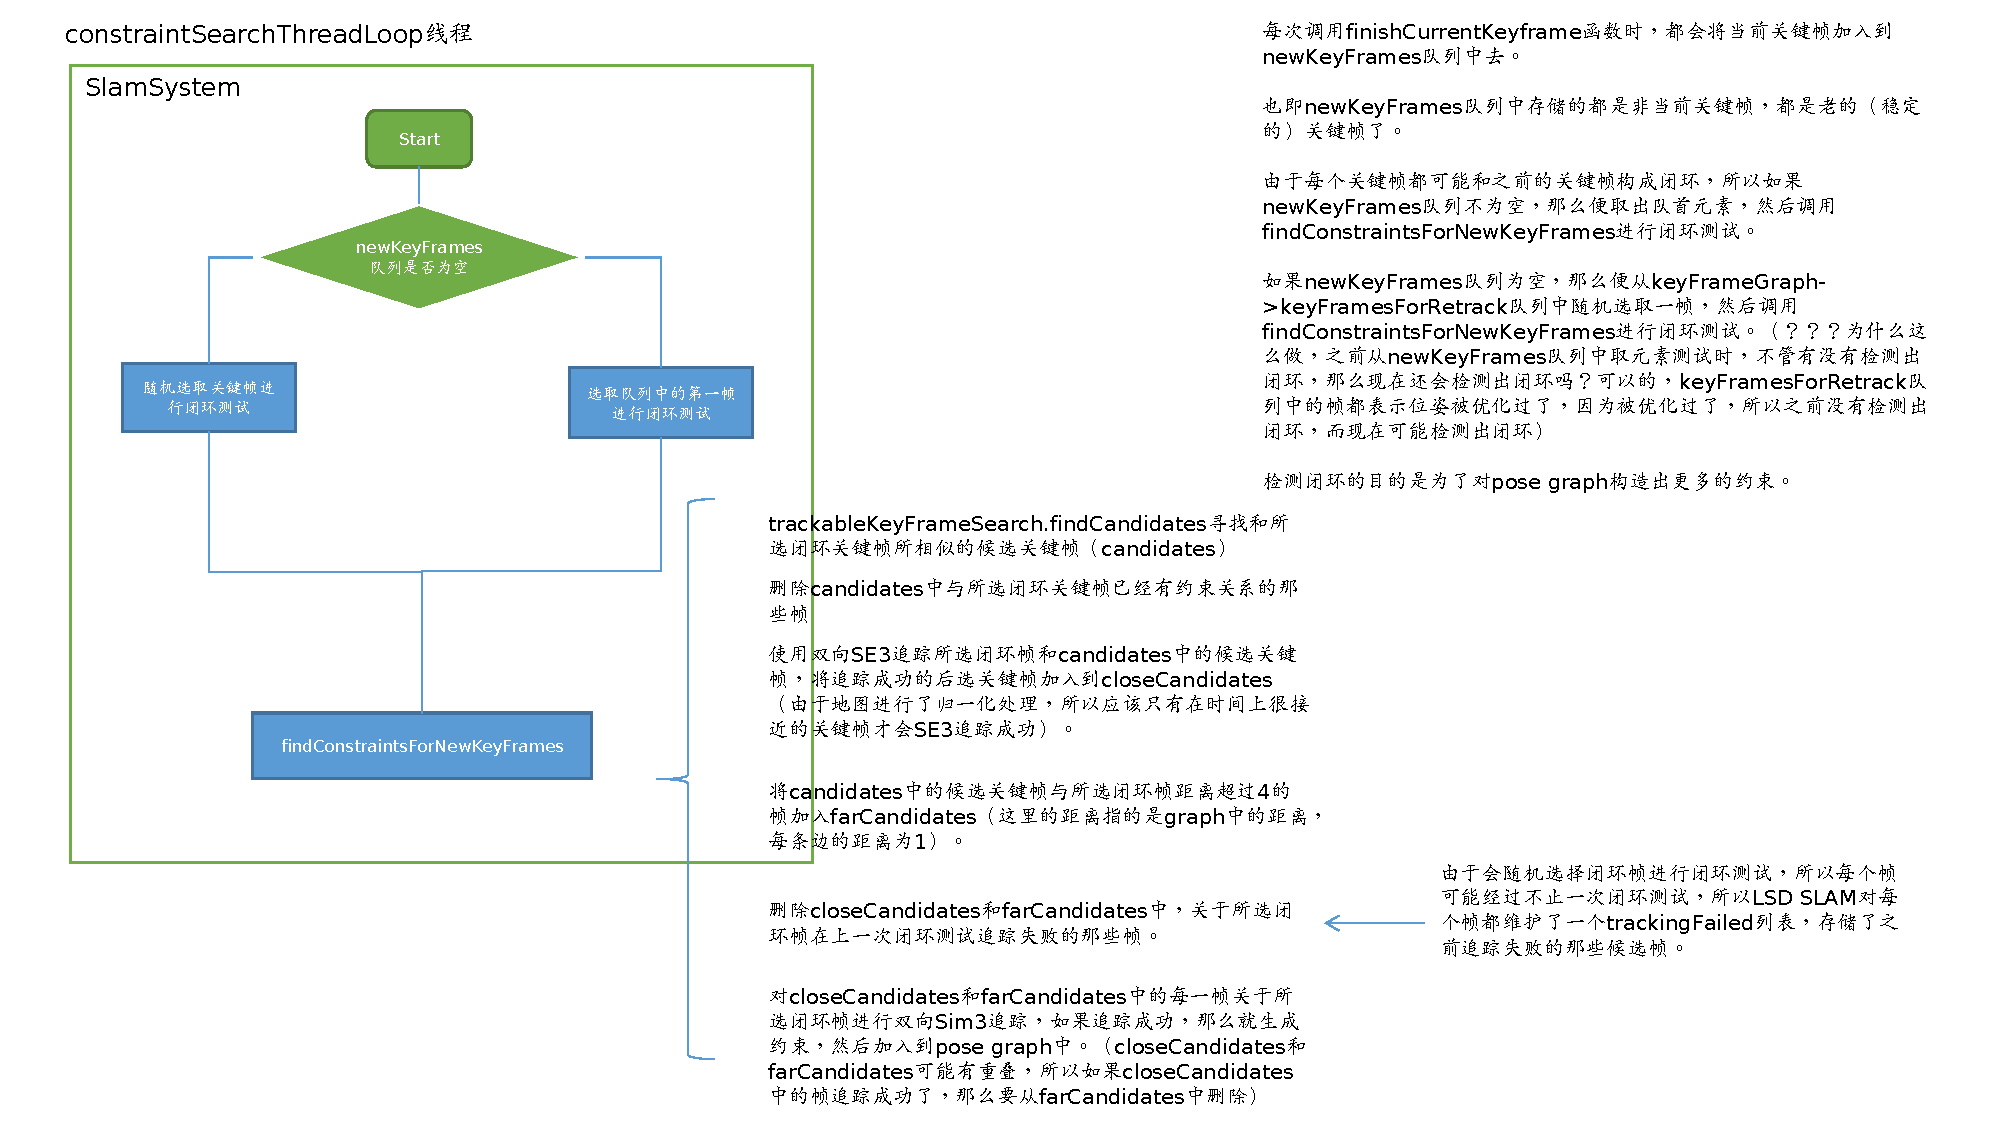
\includegraphics[width=1.0\linewidth]{image/LSD-SLAM/LSD-SLAM-constraint.pdf}  %插入的图,包括JPG,PNG,PDF,EPS等,放在源文件目录下
	\caption{constraintSearchThreadLoop流程图.}  %图片的名称
	\label{fig:constraint_search_thread}   %标签,用作引用
\end{figure}



\section{Optimization}

优化的话,就是对之前构建的pose graph进行优化。
\begin{figure}[h]%%图
	\centering  %插入的图片居中表示
	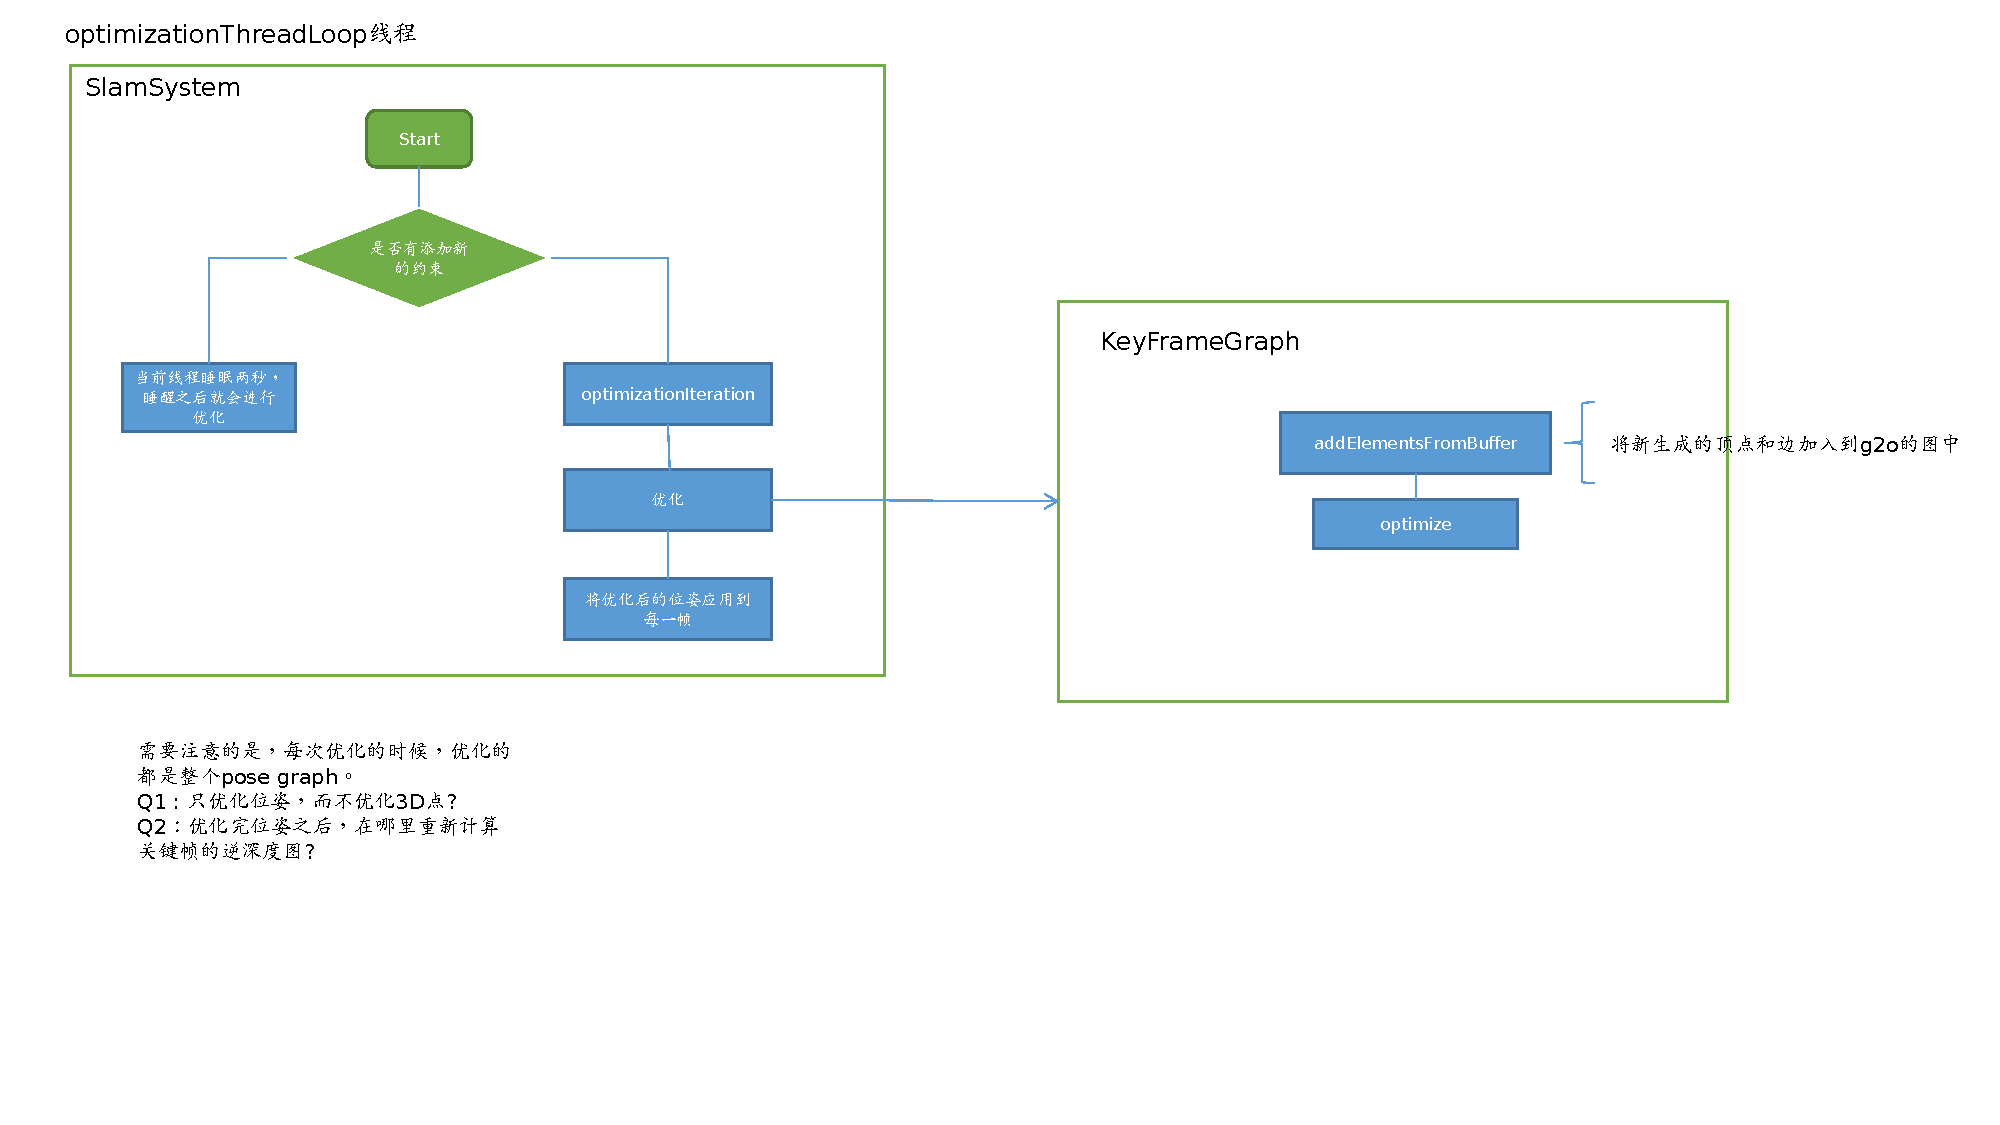
\includegraphics[width=1.0\linewidth]{image/LSD-SLAM/LSD-SLAM-optimization.pdf}  %插入的图,包括JPG,PNG,PDF,EPS等,放在源文件目录下
	\caption{optimizationThread流程图.}  %图片的名称
	\label{fig:optimization_thread}   %标签,用作引用
\end{figure}